%%%%%%%%%%%%%%%%%%%%%%%%%%%%%%%%%%%%%%%%%
% Stylish Article
% LaTeX Template
% Version 2.0 (13/4/14)
%
% This template has been downloaded from:
% http://www.LaTeXTemplates.com
%
% Original author:
% Mathias Legrand (legrand.mathias@gmail.com)
%
% License:
% CC BY-NC-SA 3.0 (http://creativecommons.org/licenses/by-nc-sa/3.0/)
%
%%%%%%%%%%%%%%%%%%%%%%%%%%%%%%%%%%%%%%%%%

%----------------------------------------------------------------------------------------
%	PACKAGES AND OTHER DOCUMENT CONFIGURATIONS
%----------------------------------------------------------------------------------------

\documentclass[fleqn,10pt]{SelfArx} % Document font size and equations flushed left

\usepackage{lipsum} % Required to insert dummy text. To be removed otherwise


%----------------------------------------------------------------------------------------
%	Source Code Listings
%----------------------------------------------------------------------------------------
\usepackage{listings}
\usepackage{xcolor}
\definecolor{darkgreen}{rgb}{0.0, 0.2, 0.13}
\definecolor{ao}{rgb}{0.0, 0.5, 0.0}
\lstdefinestyle{sharpc}{language=[Sharp]C, frame=single}
\lstset{% general command to set parameter(s)
basicstyle=\small, % print whole listing small
keywordstyle=\color{blue}\bfseries,
% underlined bold black keywords
commentstyle=\small\color{ao}, % white comments
stringstyle=\ttfamily, % typewriter type for strings
columns=fullflexible, % keeps the comments from exploding
showstringspaces=false} % no special string spaces


%----------------------------------------------------------------------------------------
%	COLUMNS
%----------------------------------------------------------------------------------------

\setlength{\columnsep}{0.55cm} % Distance between the two columns of text
\setlength{\fboxrule}{0.75pt} % Width of the border around the abstract

%----------------------------------------------------------------------------------------
%	COLORS
%----------------------------------------------------------------------------------------

\definecolor{color1}{RGB}{0,0,90} % Color of the article title and sections
\definecolor{color2}{RGB}{0,20,20} % Color of the boxes behind the abstract and headings

%----------------------------------------------------------------------------------------
%	HYPERLINKS
%----------------------------------------------------------------------------------------

\usepackage{hyperref} % Required for hyperlinks
\hypersetup{hidelinks,colorlinks,breaklinks=true,urlcolor=color2,citecolor=color1,linkcolor=color1,bookmarksopen=false,pdftitle={Title},pdfauthor={Author}}

%----------------------------------------------------------------------------------------
%	ARTICLE INFORMATION
%----------------------------------------------------------------------------------------

\JournalInfo{PBIP \#78, 2015} % Journal information
\Archive{Additional note} % Additional notes (e.g. copyright, DOI, review/research article)

\PaperTitle{PacBio Improvement Proposal \#((int)`N') \\{\large Removing the deletion tag value from secondary analysis}} % Article title

\Authors{Nigel Delaney} % Authors

\Keywords{} % Keywords - if you don't want any simply remove all the text between the curly brackets
\newcommand{\keywordname}{Keywords} % Defines the keywords heading name

%----------------------------------------------------------------------------------------
%	ABSTRACT
%----------------------------------------------------------------------------------------

\Abstract{ The PacBio consensus calling framework is greatly complicated by the presence of deletion tag values attached to certain basepairs.  These  that are emitted by the .}

%----------------------------------------------------------------------------------------

\begin{document}

\flushbottom % Makes all text pages the same height

\maketitle % Print the title and abstract box

\tableofcontents % Print the contents section

\thispagestyle{empty} % Removes page numbering from the first page

%----------------------------------------------------------------------------------------
%	ARTICLE CONTENTS
%----------------------------------------------------------------------------------------

\section*{Introduction} % The \section*{} command stops section numbering

\addcontentsline{toc}{section}{Introduction} % Adds this section to the table of contents

A desirable statistical model is no more complex than necessary, does not contain unnecessary parameters and has a likelihood function that is smooth and continuous to aid in optimization.  There should also be a well defined generative process that defines how the observed data should be interpreted.

The use of Deletion Tags (DelTags), in secondary analysis takes the CCS and Quiver models further away from, rather than closer to, this ideal.  The proposal suggests that either DelTag values should be removed entirely, or the deleted base should be promoted to an actual base in the read sequence, so that it could be handled using the framework for insertions/deletions already present in the scoring models that does not require DelTag values. 

Here, I review the origin and rational for deletions tags then present several arguments for their removal. 



\subsection{What are DelTags?}
Each base in a PacBio dataset may have an associated DelTag value which is one of the basepairs A, C, G, T.  It is defined in the PacBio documentation as the \textit{``Likely identity of a deleted base, if it exists"}.  In practice, typically approximately 10\% of bases in a dataset will have this value, the remainder will have a `N' value.  However the percentage of bases with a DelTag varies by overall read quality as shown in Figure \ref{fig:RateByRQ}\footnote{Generated using code in ExamineDelTags.fs and ExamineDelTags.R.}.  The DeletionTag value is created within the method that converts pulses into bases\footnote{Method: \texttt{ AnalyzeInsertClassify@PulseToBaseStream.cs:521}}.

\begin{figure}[ht]\centering 
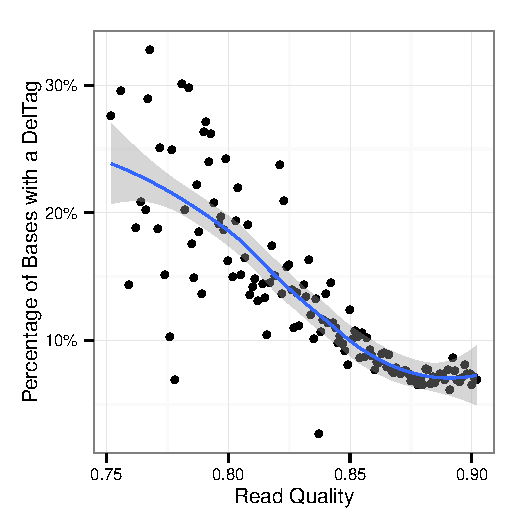
\includegraphics[width=\linewidth]{TagRateByRQ}
\caption{DelTag Appearance Rate by Read Quality.  Each dot represents the average percentage of non `N' DelTags that appeared in reads with the RQ value given by the position along the x-axis. }
\label{fig:RateByRQ}
\end{figure}


Before discussing when and how DelTags are added, it is worth mentioning that generally speaking, the Deletion QV values emitted from PacBio data processing are not very useful, and their calculation appears to be an unfinished project.  It appears Pat originally intended to create Deletion QV values using a GBM\footnote{Generalized Boosted Model, for more details see the R package GBM.} to predict the likelihood of error, as is currently done for insertion QVs.  However, at present the values for the deletion QV are all hardcoded to a QV of 17 with the following line of code:\footnote{\texttt{PulseToBaseStream.cs:478}}

\lstset{style=sharpc}
\begin{lstlisting}[frame=single]
/* This could be done much more intelligently.
  We weren't really able to get a DeletionClassifier
  to give much benefit. */
delPrediction = incPredictions.Map(v => 0.02f);
\end{lstlisting}

Although all DeletionQV values are initially hard-coded to the seemingly arbitrary 17 value in PulseToBases, this value can later be modified if and only if when converting pulses to bases some pulses are not emitted, or are skipped.  If a pulse is skipped, then a new DeletionQV value, and a DelTag, is attached to the next pulse converted to a base.  This is the only time a DelTag will exist.

To obtain both the base and the QV value, the skipped pulses are all evaluated.  The basepair of the skipped pulse with the highest probability of incorporation becomes the DelTag basepair.  A new DeletionQV value is then calculated as the sum of all the deletion probabilities for the skipped pulses (which are all a fixed constant), plus the probability of incorporation for the most likely base.  The specific code to do this is shown below.\footnote{\texttt{PulseToBaseStream.cs:636}}

\lstset{style=sharpc}
\begin{lstlisting}[frame=single]
// sum up all the deletion probability since the last base
float dqvs1 = 0.0;
// We did skip some pulses since the last base
// For now lets just consider the one that was closest to being a base
float skippedIncMax = float.MinValue;
int worstSkippedPulseIndex = 0;
// This could use a bit of attention
foreach(var p in skippedPulses) {
    if(incPredictions[p] > skippedIncMax)    {
        skippedIncMax = incPredictions[p];
        worstSkippedPulseIndex = p;
    }
    dqvs1 += delPredictions[p];
}
/*  Total probability of a deletion is the sum of the bg deletion rates 
over the gaps, plus the incorporation probability of the leftover 
pulse. */
delProb = dqvs1 + incPredictions[worstSkippedPulseIndex];
delQV.Add(QVs.ProbToQV(delProb));
delTag.Add(iBases[worstSkippedPulseIndex]);
\end{lstlisting}

The algorithm in this code is wrong for several reasons.  First, when considering deletion events before each pulse, this code sums the deletion probabilities before each pulse that is skipped. The correct calculation, given the fixed value of 0.02 for $N$ skipped pulses would be to account for the probability that there were no deletions before each pulse as: $ (1 - (1-.02)^N)$.  Fortunately (or perhaps by uncommented design), because the fixed constant currently used as the default deletion probability is small, the summation used and the correct formula should often give similar results as $(1-0.02)^N \thickapprox 1 - N\cdot0.02$.  However, this will not generally be true for larger fixed constants and/or a large number of skipped pulses.

The second issue is that only the pulse with the highest probability of being a true incorporation is considered.  The correct formula for multiple skipped pulses would be similar to the one given in the last paragraph, but replacing the fixed constant with the value for each pulse's incorporation probability.  As before, the calculation currently used may approximate the correct value under some conditions, in particular if there is only one skipped pulse or if only one pulse has any meaningful incorporation probability.  Also as before, these conditions may not always hold. 


 



%------------------------------------------------

\section{Principled Arguments Against DelTags}



\subsection{They make scoring complex}

The ``Deletion Move" in our template scoring routine is done in one of two distinct ways depending on if a Deletion Tag is present.  With positions denoted by Figure \ref{fig:del}, a Deletion move is currently scored according to the equation shown below.  

\begin{figure}[ht]\centering % Using \begin{figure*} makes the figure take up the entire width of the page
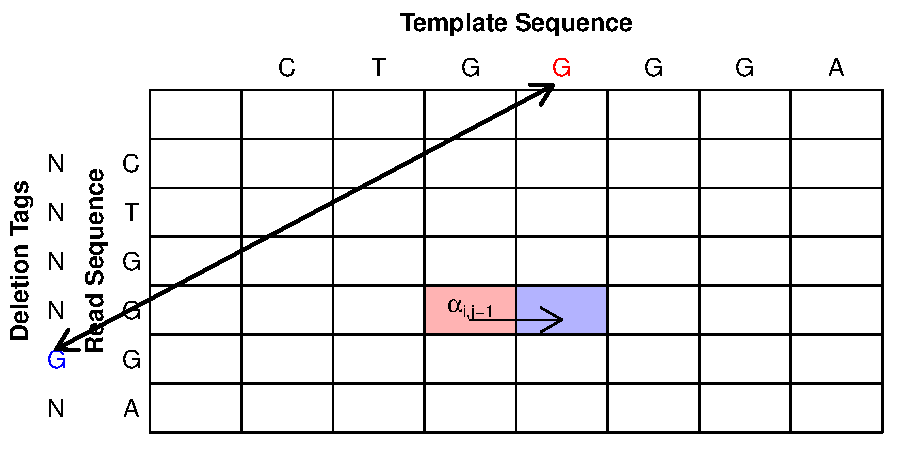
\includegraphics[width=\linewidth]{Deletion}
\caption{Deletion Scoring}
\label{fig:del}
\end{figure}

\[
	\alpha_{i,j-1}  +  \begin{cases}
							 \text{Deletion score  for } R_{i+1}  & \text{if }  \text{DeletionTag}_{i+1} = T_{j} \\
							 \text{A fixed constant} & \text{if }  \text{DeletionTag}_{i+1} \neq T_{j} 
							 \end{cases}
\]

By having two possible scoring methods, we not only need to estimate 3 parameters for the deletion move in training, but we also are scoring the same behavior (a deletion in the template), using two separate methods.

\subsection{Knowing the identity of the base most likely to have been deleted should not add value.}

The algorithm should be able to ignore the specific base specified by the DelTag and work just as well.  Here's why: If the sequence \texttt{GGGG} was accidentally emitted as \texttt{GGG} due to a pulse with a `G' being skipped and emitted as a DelTag, we would not expect the other reads from this template to generate odd sequences with a random base inserted,  such as \texttt{GGAG} or \texttt{GGCG}.  Because single read PacBio data is correct $\sim87\%$ of the time, instead we would expect most of the other reads we consider to represent the true sequence, i.e. \texttt{GGGG}.  In general, when generating a consensus with multiple reads we will always be debating between the true sequence and a sequence close to truth, i.e. \texttt{GGGG} versus \texttt{GGG}.

As a consequence of this, with multiple reads being used to generate a consensus, the algorithm can and will determine what the most likely alternate base was using the other reads, not the DelTag.  If \texttt{GGGG} shows up in several reads, we should expect and hope that the reads with \texttt{GGG} contain a DeletionTag with a value of `G'.  It would be an improbable world if by ignoring the DelTag value, the algorithm accepted the sequence \texttt{GGGG} over \texttt{GGG} only because it weighed several DelTag values and assumed they were `G' even though they were `A', `C', or `T'. 

In other words, \textit{we don't need to encode the most likely deleted base in the DelTag because it is already encoded by the other reads used for consensus}. 
 


\subsection{Subsection}

\lipsum[6] % Dummy text

\paragraph{Paragraph} \lipsum[7] % Dummy text
\paragraph{Paragraph} \lipsum[8] % Dummy text

\subsection{Subsection}

\lipsum[9] % Dummy text




%------------------------------------------------

\section{Empirical Arguments Against DelTags}

\subsection{They are rarely correct.}

The overall rate at which a DelTag is correct is only $\sim3.6\%$ and this value does not improve much based on read quality as can be seen in Figure \ref{fig:rateCorrect}.  


\begin{figure}[ht]\centering
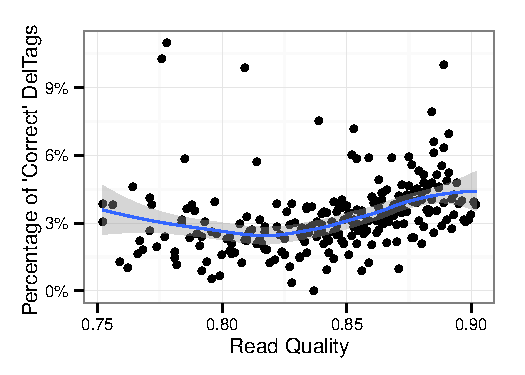
\includegraphics[width=\linewidth]{TagCorrectRateByRQ.pdf}
\caption{Percentage of DelTags Correct by RQ.  For each DelTag in an aligned set of subreads, I counted the DelTag as correct if it followed a deletion of the given base in the alignment (with some accounting for different alignments within homopolymers).  Each dot in this graph represents the average for a set of subreads binned by RQ. For more details, see the cafe-quality commit  }
\label{fig:rateCorrect}
\end{figure}


%------------------------------------------------

\section{Results and Discussion}

\lipsum[10] % Dummy text

\subsection{Subsection}

\lipsum[11] % Dummy text

\begin{table}[hbt]
\caption{Table of Grades}
\centering
\begin{tabular}{llr}
\toprule
\multicolumn{2}{c}{Name} \\
\cmidrule(r){1-2}
First name & Last Name & Grade \\
\midrule
John & Doe & $7.5$ \\
Richard & Miles & $2$ \\
\bottomrule
\end{tabular}
\label{tab:label}
\end{table}

\subsubsection{Subsubsection}

\lipsum[12] % Dummy text

\begin{description}
\item[Word] Definition
\item[Concept] Explanation
\item[Idea] Text
\end{description}

\subsubsection{Subsubsection}

\lipsum[13] % Dummy text

\begin{itemize}[noitemsep] % [noitemsep] removes whitespace between the items for a compact look
\item First item in a list
\item Second item in a list
\item Third item in a list
\end{itemize}

\subsubsection{Subsubsection}

\lipsum[14] % Dummy text

\subsection{Subsection}

\lipsum[15-23] % Dummy text


\section{Conclusions}
A statistical model with additional parameters and/or information can always beat a simpler model.  Simpler models provide alternate benefits in that they are easier to analyze, more tractable computationally, and 



%------------------------------------------------
\phantomsection
\section*{Acknowledgments} % The \section*{} command stops section numbering

\addcontentsline{toc}{section}{Acknowledgments} % Adds this section to the table of contents

So long and thanks for all the fish \cite{Figueredo:2009dg}.

%----------------------------------------------------------------------------------------
%	REFERENCE LIST
%----------------------------------------------------------------------------------------
\phantomsection
\bibliographystyle{unsrt}
\bibliography{sample}

%----------------------------------------------------------------------------------------

\end{document}